\ifdefined\included
\else
\documentclass[english,a4paper,11pt,twoside]{StyleThese}
\usepackage{amsmath,amssymb}             % AMS Math
\usepackage[T1]{fontenc}
\usepackage[utf8x]{inputenc}
\usepackage{babel}
\usepackage{datetime}

\usepackage{lmodern}
\usepackage{tabularx}
%\usepackage{tabular}
\usepackage{multirow}

\usepackage{subfigure}
\usepackage{fancyvrb}


\usepackage{hhline}
\usepackage[left=1.5in,right=1.3in,top=1.1in,bottom=1.1in,includefoot,includehead,headheight=13.6pt]{geometry}
\renewcommand{\baselinestretch}{1.05}

% Table of contents for each chapter

\usepackage[nottoc, notlof, notlot]{tocbibind}
\usepackage{minitoc}
\setcounter{minitocdepth}{2}
\mtcindent=15pt
% Use \minitoc where to put a table of contents

\usepackage{aecompl}


% Glossary / list of abbreviations

\usepackage[intoc]{nomencl}
\iftoggle{ThesisInEnglish}{%
\renewcommand{\nomname}{Glossary}
}{ %
\renewcommand{\nomname}{Liste des Abréviations}
}

\makenomenclature

% My pdf code

\usepackage{ifpdf}

\ifpdf
  \usepackage[pdftex]{graphicx}
  \DeclareGraphicsExtensions{.jpg}
  \usepackage[a4paper,pagebackref,hyperindex=true]{hyperref}
  \usepackage{tikz}
  \usetikzlibrary{arrows,shapes,calc}
\else
  \usepackage{graphicx}
  \DeclareGraphicsExtensions{.ps,.eps}
  \usepackage[a4paper,dvipdfm,pagebackref,hyperindex=true]{hyperref}
\fi

\graphicspath{{.}{images/}}

%% nicer backref links. NOTE: The flag ThesisInEnglish is used to define the
% language in the back references. Read more about it in These.tex

\iftoggle{ThesisInEnglish}{%
\renewcommand*{\backref}[1]{}
\renewcommand*{\backrefalt}[4]{%
\ifcase #1 %
(Not cited.)%
\or
(Cited in page~#2.)%
\else
(Cited in pages~#2.)%
\fi}
\renewcommand*{\backrefsep}{, }
\renewcommand*{\backreftwosep}{ and~}
\renewcommand*{\backreflastsep}{ and~}
}{%
\renewcommand*{\backref}[1]{}
\renewcommand*{\backrefalt}[4]{%
\ifcase #1 %
(Non cité.)%
\or
(Cité en page~#2.)%
\else
(Cité en pages~#2.)%
\fi}
\renewcommand*{\backrefsep}{, }
\renewcommand*{\backreftwosep}{ et~}
\renewcommand*{\backreflastsep}{ et~}
}

% Links in pdf
\usepackage{color}
\definecolor{linkcol}{rgb}{0,0,0.4} 
\definecolor{citecol}{rgb}{0.5,0,0} 
\definecolor{linkcol}{rgb}{0,0,0} 
\definecolor{citecol}{rgb}{0,0,0}
% Change this to change the informations included in the pdf file

\hypersetup
{
bookmarksopen=true,
pdftitle="Joint Action for Human-Robot Interaction",
pdfauthor="Sandra DEVIN", %auteur du document
pdfsubject="Thesis", %sujet du document
%pdftoolbar=false, %barre d'outils non visible
pdfmenubar=true, %barre de menu visible
pdfhighlight=/O, %effet d'un clic sur un lien hypertexte
colorlinks=true, %couleurs sur les liens hypertextes
pdfpagemode=None, %aucun mode de page
pdfpagelayout=SinglePage, %ouverture en simple page
pdffitwindow=true, %pages ouvertes entierement dans toute la fenetre
linkcolor=linkcol, %couleur des liens hypertextes internes
citecolor=citecol, %couleur des liens pour les citations
urlcolor=linkcol %couleur des liens pour les url
}

% definitions.
% -------------------

\setcounter{secnumdepth}{3}
\setcounter{tocdepth}{2}

% Some useful commands and shortcut for maths:  partial derivative and stuff

\newcommand{\pd}[2]{\frac{\partial #1}{\partial #2}}
\def\abs{\operatorname{abs}}
\def\argmax{\operatornamewithlimits{arg\,max}}
\def\argmin{\operatornamewithlimits{arg\,min}}
\def\diag{\operatorname{Diag}}
\newcommand{\eqRef}[1]{(\ref{#1})}

\usepackage{rotating}                    % Sideways of figures & tables
%\usepackage{bibunits}
%\usepackage[sectionbib]{chapterbib}          % Cross-reference package (Natural BiB)
%\usepackage{natbib}                  % Put References at the end of each chapter
                                         % Do not put 'sectionbib' option here.
                                         % Sectionbib option in 'natbib' will do.
\usepackage{fancyhdr}                    % Fancy Header and Footer

% \usepackage{txfonts}                     % Public Times New Roman text & math font
  
%%% Fancy Header %%%%%%%%%%%%%%%%%%%%%%%%%%%%%%%%%%%%%%%%%%%%%%%%%%%%%%%%%%%%%%%%%%
% Fancy Header Style Options

\pagestyle{fancy}                       % Sets fancy header and footer
\fancyfoot{}                            % Delete current footer settings

%\renewcommand{\chaptermark}[1]{         % Lower Case Chapter marker style
%  \markboth{\chaptername\ \thechapter.\ #1}}{}} %

%\renewcommand{\sectionmark}[1]{         % Lower case Section marker style
%  \markright{\thesection.\ #1}}         %

\fancyhead[LE,RO]{\bfseries\thepage}    % Page number (boldface) in left on even
% pages and right on odd pages
\fancyhead[RE]{\bfseries\nouppercase{\leftmark}}      % Chapter in the right on even pages
\fancyhead[LO]{\bfseries\nouppercase{\rightmark}}     % Section in the left on odd pages

\let\headruleORIG\headrule
\renewcommand{\headrule}{\color{black} \headruleORIG}
\renewcommand{\headrulewidth}{1.0pt}
\usepackage{colortbl}
\arrayrulecolor{black}

\fancypagestyle{plain}{
  \fancyhead{}
  \fancyfoot{}
  \renewcommand{\headrulewidth}{0pt}
}

%\usepackage{MyAlgorithm}
%\usepackage[noend]{MyAlgorithmic}
\usepackage[ED=MITT - STICIA, Ets=INP]{tlsflyleaf}
%%% Clear Header %%%%%%%%%%%%%%%%%%%%%%%%%%%%%%%%%%%%%%%%%%%%%%%%%%%%%%%%%%%%%%%%%%
% Clear Header Style on the Last Empty Odd pages
\makeatletter

\def\cleardoublepage{\clearpage\if@twoside \ifodd\c@page\else%
  \hbox{}%
  \thispagestyle{empty}%              % Empty header styles
  \newpage%
  \if@twocolumn\hbox{}\newpage\fi\fi\fi}

\makeatother
 
%%%%%%%%%%%%%%%%%%%%%%%%%%%%%%%%%%%%%%%%%%%%%%%%%%%%%%%%%%%%%%%%%%%%%%%%%%%%%%% 
% Prints your review date and 'Draft Version' (From Josullvn, CS, CMU)
\newcommand{\reviewtimetoday}[2]{\special{!userdict begin
    /bop-hook{gsave 20 710 translate 45 rotate 0.8 setgray
      /Times-Roman findfont 12 scalefont setfont 0 0   moveto (#1) show
      0 -12 moveto (#2) show grestore}def end}}
% You can turn on or off this option.
% \reviewtimetoday{\today}{Draft Version}
%%%%%%%%%%%%%%%%%%%%%%%%%%%%%%%%%%%%%%%%%%%%%%%%%%%%%%%%%%%%%%%%%%%%%%%%%%%%%%% 

\newenvironment{maxime}[1]
{
\vspace*{0cm}
\hfill
\begin{minipage}{0.5\textwidth}%
%\rule[0.5ex]{\textwidth}{0.1mm}\\%
\hrulefill $\:$ {\bf #1}\\
%\vspace*{-0.25cm}
\it 
}%
{%

\hrulefill
\vspace*{0.5cm}%
\end{minipage}
}

\let\minitocORIG\minitoc
\renewcommand{\minitoc}{\minitocORIG \vspace{1.5em}}

\usepackage{multirow}
%\usepackage{slashbox}

\newenvironment{bulletList}%
{ \begin{list}%
	{$\bullet$}%
	{\setlength{\labelwidth}{25pt}%
	 \setlength{\leftmargin}{30pt}%
	 \setlength{\itemsep}{\parsep}}}%
{ \end{list} }

\newtheorem{definition}{Définition}
\renewcommand{\epsilon}{\varepsilon}

% centered page environment

\newenvironment{vcenterpage}
{\newpage\vspace*{\fill}\thispagestyle{empty}\renewcommand{\headrulewidth}{0pt}}
{\vspace*{\fill}}

\usepackage{tablefootnote}

\sloppy
\begin{document}
\setcounter{chapter}{0} %% Numéro du chapitre précédent ;)
\dominitoc
\faketableofcontents
\fi

\chapter{From Human-Human Joint Action to Human-Robot Joint Action}
\minitoc

\section{Joint Action Theory}

A first step to endow robots with the ability to perform Joint Actions with humans is to understand how humans act together. As a working definition of Joint Action, we will use the one from \cite{sebanz2006joint}:

\begin{quote}
\textit{Joint action can be regarded as any form of social interaction whereby two or more individuals coordinate their actions in space and time to bring about a change in the environment.}
\end{quote}

A given number of prerequisites are needed for these individuals to achieve the so-called Joint Action. First of all, they need to agree on the change they want to bring in the environment, the conditions under which they will stay engaged in its realisation and the way to do it. A number of works have studied this prerequisite, named \textit{commitment}, which I will develop in Sec.~\ref{subsec:commitment}. Then, as mentioned in the definition, the individuals need to coordinate their actions in space and time. This will be studied in Sec.~\ref{subsec:coordination}. Finally, in order to coordinate, each individual needs to be aware of the other, he needs to be able to perceive him and predict his actions. This part will be develop in Sec.~\ref{subsec:prediction}.

\subsection{Commitment}

\label{subsec:commitment}

The first prerequisite to achieve a Joint Action is to have a \textit{goal} to pursue and the \textit{intention} to achieve it. Let's define in a first time what is called a \textit{goal} and an \textit{intention} for a single person before going to a \textit{joint goal} and a \textit{joint intention}.

In \cite{tomasello2005understanding}, Tomasello et al. define what they call a \textit{goal} and an \textit{intention} and illustrate these definitions with an example and an associated figure (fig.~\ref{fig:intention}) where a person wants to open a box.

\begin{figure}[!h]
	\centering
    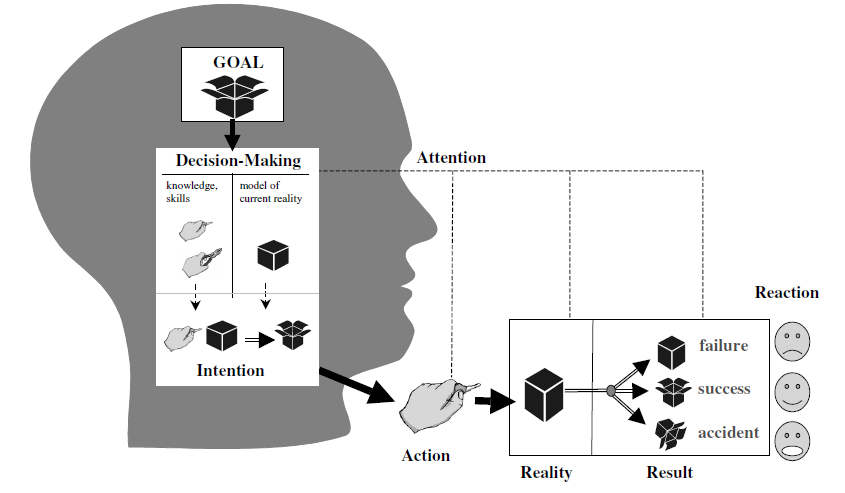
\includegraphics[width=0.8\textwidth]{figs/Chapter1/intention.png}
    \caption{Illustrative example of an intentional action by Tomasello et al. Here the human has for \textit{goal} to open the box. He chooses a means to perform it and so forms an \textit{intention}.}
    \label{fig:intention}
\end{figure}

A \textit{goal} is defined here as the representation of the desired state by the agent (in the example, the goal is an open box) and, based on Bratman's work \cite{bratman1989intention}, an \textit{intention} is defined as an action plan the agent commits itself in pursuit of a goal (in the example, the intention is to use a key to open the box). The \textit{intention} includes both a \textit{goal} and the means to achieve it. 

In a same way, Cohen and Levesque propose in \cite{cohen1991teamwork} a formal definition of what they call a \textit{persistent goal}:

\begin{quote}
\textbf{Definition: } An agent has a \textit{persistent goal} relative to \textit{q} to achieve \textit{p} iff:
\begin{enumerate}
\item she believes that \textit{p} is currently false;
\item she wants \textit{p} to be true eventually;
\item it is true (and she knows it) that (2) will continue to hold until she comes to believe either that \textit{p} is true, or that it will neither be true, or that \textit{q} is false.
\end{enumerate}
\end{quote}

However, their definition of an \textit{intention} differs a little from the previous one. They define an \textit{intention} as a commitment to act in a certain mental state:

\begin{quote}
\textbf{Definition:} An agent \textit{intends} relative to some conditions to do an action just in case she has a persistent goal (relative to that condition) of having done the action, and, moreover, having done it, believing throughout that she is doing it.
\end{quote}

The \textit{intention} still includes the \textit{goal} but here it concerns more the fact that the agent commits itself to achieve the goal than the way to achieve it.

Let's now apply these principles to a Joint Action. One of the most known definition of \textit{joint intention} is the one of Bratman \cite{bratman1993shared}:

\begin{quote}
We intend to \textit{J} if and only if:
\begin{enumerate}
\item (a) I intend that we \textit{J} and (b) you intend that we \textit{J}.
\item I intend that we \textit{J} in accordance with and because of 1\textit{a}, 1\textit{b}, and meshing subplans of 1\textit{a} and 1\textit{b}; you intend that we \textit{J} in accordance with and because of 1\textit{a}, 1\textit{b}, and meshing subplans of 1\textit{a} and 1\textit{b}.
\item 1 and 2 are common knowledge between us.
\end{enumerate}
\end{quote}

This definition is taking back and illustrated by Tomasello et al. in \cite{tomasello2005understanding} where they reuse the example of the box to open (fig~\ref{fig:intention_jointe}).

\begin{figure}[!h]
	\centering
    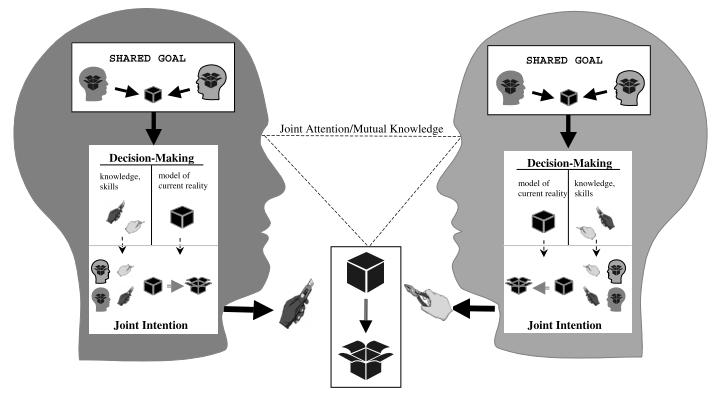
\includegraphics[width=0.8\textwidth]{figs/Chapter1/intention_jointe.png}
    \caption{Illustrative example of a collaborative activity by Tomasello et al. Here the humans have for \textit{shared goal} to open the box together. They choose a means to perform it which takes into account the other capabilities and so form a \textit{joint intention}.}
    \label{fig:intention_jointe}
\end{figure}

The \textit{shared goal} is defined as the representation of a desired state plus the fact that it will be done in collaboration with other person(s) (in the example, they will open the box together) and a \textit{joint intention} is defined as a collaborative plan the agents commit to in order to achieve the \textit{shared goal} and which takes into account both agents individual plans (here an agent will hold the box with the clamp while the other open it with the cutter).

In a same way, Cohen and Levesque extend their definition of \textit{persistent goal} and \textit{intention} to a collaborative activity. They first define a \textit{weak achievement goal} as:
\begin{quote}
\textbf{Definition: } An agent has a \textit{weak achievement goal} relative to \textit{q} and with respect to a team to bring about \textit{p} if either of these conditions holds:
\begin{itemize}
\item The agent has a normal achievement goal to bring about \textit{p}, that is, the agent does not yet believe that \textit{p} is true and has \textit{p} eventually being true as goal.
\item The agent believes that \textit{p} is true, will never be true, or is irrelevant (that is, \textit{q} is false), \textit{but} has as a goal that the status of \textit{p} be mutually believed by all the team members.
\end{itemize}
\end{quote}

They then use this definition to define a \textit{joint persistent goal}:
\begin{quote}
\textbf{Definition: } A team of agents have a \textit{joint persistent goal} relative to \textit{q} to achieve \textit{p} just in case
\begin{itemize}
\item they mutually believe that \textit{p} is currently false;
\item they mutually know they all want \textit{p} to eventually be true;
\item it is true (and mutual knowledge) that until they come to mutually believe that \textit{p is true}, that \textit{p} will never be true, or that \textit{q} is false, they will continue to mutually believe that they each have \textit{p} as a weak achievement goal relative to \textit{q} and with respect to the team.
\end{itemize}
\end{quote}

They finally define a \textit{joint intention} as:
\begin{quote}
\textbf{Definition:} A team of agents \textit{jointly intends}, relative to some escape condition, to do an action iff the members have a joint persistent goal relative of that condition of their having done the action and, moreover, having done it mutually believing throughout that they were doing it.
\end{quote}

As previously, the definitions of Cohen and Levesque do no take into account the way to achieve the \textit{shared goal}, however, they introduce the interesting idea that agents are also engaged to communicate about the state of the \textit{shared goal}.

Concerning the way to achieve a \textit{shared goal}, mentioned into the definition of the \textit{joint intention} of Tomasello et al., Grosz and Sidner initially introduce and formalize the notion of \textit{Shared Plan} in \cite{grosz1988plans}, which is extended in \cite{grosz1999evolution}. The key properties of their model are as follows:
\begin{quote}
\begin{enumerate}
\item it uses individual intentions to establish commitment of collaborators to their joint activity
\item it establishes an agent's commitments to its collaborating partners' abilities to carry out their
individual actions that contribute to the joint activity
\item it accounts for helpful behavior in the context of collaborative activity
\item it covers contracting actions and distinguishes contracting from collaboration
\item the need for agents to communicate is derivative, not stipulated, and follows from the general
commitment to the group activity
\item the meshing of subplans is ensured it is also derivative from more general constraints.
\end{enumerate}
\end{quote}

With their definition, each agent does not necessarily know the all \textit{Shared Plan} but only his own individual plan and the meshing subparts of the plan. The group has a \textit{Shared Plan}, but no individual member necessarily has the whole \textit{Shared Plan}.

In conclusion, the concepts concerning the commitment of agents to a collaborative activity that we will use in this thesis can be summarized as:
\begin{itemize}
\item A \textit{goal} will be represented as a desired state.
\item A\textit{shared goal} will be considered as a \textit{goal} to be achieved in collaboration with other partner(s). An agent is considered engaged in a \textit{shared goal} if he believes the goal is currently false, he wants the goal to be true and he will not give up on the goal unless he knows that the goal is achieved, not feasible or not relevant any more and he knows that his partners are aware of it.
\item A \textit{joint intention} will include a \textit{shared goal} and the way to realize it. This way will be represented as a \textit{Shared Plan} which will take into account each agent capacities and the potential conflicts between their actions. This \textit{Shared Plan} will not be necessarily completely known by all members of the group but all individuals will know their part of the plan and the meshing subparts.
\end{itemize}


\subsection{Perception and prediction}

\label{subsec:prediction}

One important thing for an agent when performing a Joint Action is to be able to perceive and predict the actions of his partner and their effects. Based on the works in \cite{sebanz2006joint}, \cite{pacherie2011phenomenology} and \cite{obhi2011moving} we identified several necessary abilities for this predictions:

\begin{itemize}
\item \textbf{Joint attention:} The capacity for an agent to direct his attention to where the one of his partner is directed allows to share a representation of objects and events. It brings a better understanding of the other agent knowledge and where his attention is focused and so, it helps the prediction of his possible next actions. Moreover, there should be a mutual manifestation of this joint attention, meaning that we should show that we share the other attention. 
\item \textbf{Action observation:} Several studies have shown that when someone observes another person executing an action, a corresponding representation of the action is formed for the observer \cite{rizzolatti2004mirror}. This is done by what has been called the \textit{mirror-neuron} system. This behavior allows the observer to predict the outcomes of the actor's action. 
\item \textbf{Co-representation:} An agent needs to have a representation of his partner, including his goal, his capacities and the social rules he is following. Indeed, having this representation will help to predict his future actions. For example, a pedestrian who sees a red traffic light will be able to predict that the car drivers will stop. In a same way, if you know that someone is aiming to go out shopping, you will be able to predict that he will look for the key of the car.
\item \textbf{Agency:} Sometimes, when there is a close link between an action performed by oneself and an action performed by another, it can be hard to distinguish who caused a particular action effect. The capacity to attribute the action effects to the good actor is called the sense of \textit{Agency}. This sense of \textit{Agency} is an important thing in Joint Action in order to correctly predict the effects of each action.
\end{itemize}

Based on the same works as before and on \cite{sebanz2009prediction}, we can list several kinds of predictions to support Joint Action which can be done thanks to the abilities described previously :
\begin{itemize}
\item \textbf{What:} A first one is to predict what will do an agent. Two kinds of predictions can be distinguished here:
\begin{itemize}
\item \textit{action-to-goal:} this is supported by the \textit{mirror-neuron} system introduced before. Here the therm goal concerns the goal of an action, its purpose. The idea is that observing an action, it is possible to predict its goal. For example, if we observe someone extending his arm toward an object we can predict that he will pick the object.
\item \textit{goal-to-action:} here the therm goal concerns the goal of a task, as defined in the previous subsection. Knowing this goal, it can be easy to predict which action an agent will perform.
\end{itemize}
\item \textbf{When:} another prediction which is necessary is the timing of an action. Knowing when an action will occur and during how long allows to a better coordination in time.
\item \textbf{Where:} a Joint Action usually takes place in a shared space. It is therefore necessary to predict the future position of the partner and his actions in order to coordinate in space.
\end{itemize} 


\subsection{Coordination}

\label{subsec:coordination}

Knoblich \cite{knoblich20113}
\begin{itemize}
\item emergent coordination: entertainment, affordances \cite{gibson2014theory}, corrspondance action-perception, action simulation
\item planned coordination: coordination smoother (vesper, \cite{vesper2010minimal})
\end{itemize}

+communication: Clark \cite{clark1996using}

\section{How to endow a robot with Joint Action abilities}


\subsection{Engagement and Intention}

\begin{itemize}
\item Intention and plan recognition
\item Goal reasoning
\item Engagement in the task
\item human-aware task planning
\end{itemize}

\subsection{Perspective taking and humans mental states}

\begin{itemize}
\item world state management
\item perspective taking
\item mental states
\end{itemize}

\subsection{Actions realization}

\begin{itemize}
\item human-aware motion planning
\item human-aware control
\item understanding effects of actions (agency)
\end{itemize}


\subsection{Coordination}

\begin{itemize}
\item plan execution
\item dialogue
\item signalling
\item joint actions (e.g. handover)
\end{itemize}

\section{A three levels architecture}

\subsection{The three levels of Pacherie}

\cite{pacherie2008phenomenology}, \cite{pacherie2011phenomenology}

\subsection{A three levels robotics architecture}

+ related work on others robotics architecture


\ifdefined\included
\else
\bibliographystyle{StyleThese}
\bibliography{These}
\end{document}
\fi
